\documentclass[11pt,a4paper]{article}
\usepackage[T1]{fontenc}
\usepackage[utf8]{inputenc}
\usepackage[french]{babel}
\usepackage{geometry}
\usepackage{graphicx}
\usepackage{xcolor}
\usepackage{pdfpages}
\usepackage{hyperref}
\usepackage{enumitem}
\usepackage{microtype}
\geometry{margin=2.2cm}
\definecolor{stgsblue}{HTML}{173B57}
\definecolor{stgsteal}{HTML}{147D88}
\definecolor{stgslight}{HTML}{EDF5F7}
\hypersetup{colorlinks=true,linkcolor=stgsblue,urlcolor=stgsteal,pdftitle={STGS - Manuel complet d'execution et d'architecture},pdfauthor={Documentation technique STGS}}
\setlength{\parindent}{0pt}
\setlength{\parskip}{0.6em}
\begin{document}
\thispagestyle{empty}
\begin{center}
\vspace*{0.5cm}

\includegraphics[width=\textwidth]{assets/Banniere.png}
\vspace{1.4cm}
{\Huge\bfseries\color{stgsblue} STGS}\par
\vspace{0.35cm}
{\LARGE\bfseries Manuel complet d'execution et d'architecture}\par
\vspace{0.45cm}
{\large Space Telemetry Ground Station}\par
\vspace{1.0cm}
\begin{minipage}{0.86\textwidth}
\colorbox{stgslight}{\parbox{0.94\linewidth}{
\textbf{Objectif.} Ce manuel permet de suivre precisement le chemin d'execution du programme depuis chaque ligne de commande jusqu'aux fonctions C++ appelees. Il documente egalement les validations, les threads, les sockets, les formats binaires, les effets de bord, les garanties et les limites du projet.
}}
\end{minipage}
\vfill
{\large Documentation technique de revue et d'entretien}\par
\vspace{0.2cm}
\end{center}
\clearpage
\section*{Organisation du manuel}
Ce document regroupe cinq volumes complementaires. Chaque volume reste egalement disponible sous forme de source \LaTeX{} et de PDF autonome.

\begin{enumerate}[leftmargin=*,itemsep=0.8em]
  \item \textbf{Architecture et execution} -- architecture generale, format STGS/STGA, pipeline, threads, reseau, CRC et chemin d'une trame.
  \item \textbf{Commandes de la station sol} -- execution detaillee des commandes \texttt{stgs\_ground\_station}, TCP, UDP, replay, auto-port, filtres et sorties.
  \item \textbf{Commandes du simulateur} -- generation de telemetrie, messages, signaux, bruit, corruption, decouverte de ports et capture STGF.
  \item \textbf{Diagnostics, build, tests et benchmark} -- CMake, Makefile, tests, sanitizers, diagnostic de ports et benchmark de decodage.
  \item \textbf{Limites, invariants et entretien} -- bornes exactes, garanties, non-garanties, choix de conception et questions de revue technique.
\end{enumerate}

\vfill
\textbf{Convention de lecture.} Les arbres d'appels indiquent le chemin fonctionnel principal. Les noms de fonctions et de fichiers correspondent au code source du projet. Les limites chiffrees sont celles imposees par l'implementation documentee, et non des exigences normatives aerospatiales sauf mention explicite.
\clearpage

% Les volumes sont inclus tels quels afin que leur mise en page autonome et leurs references de code restent intactes.
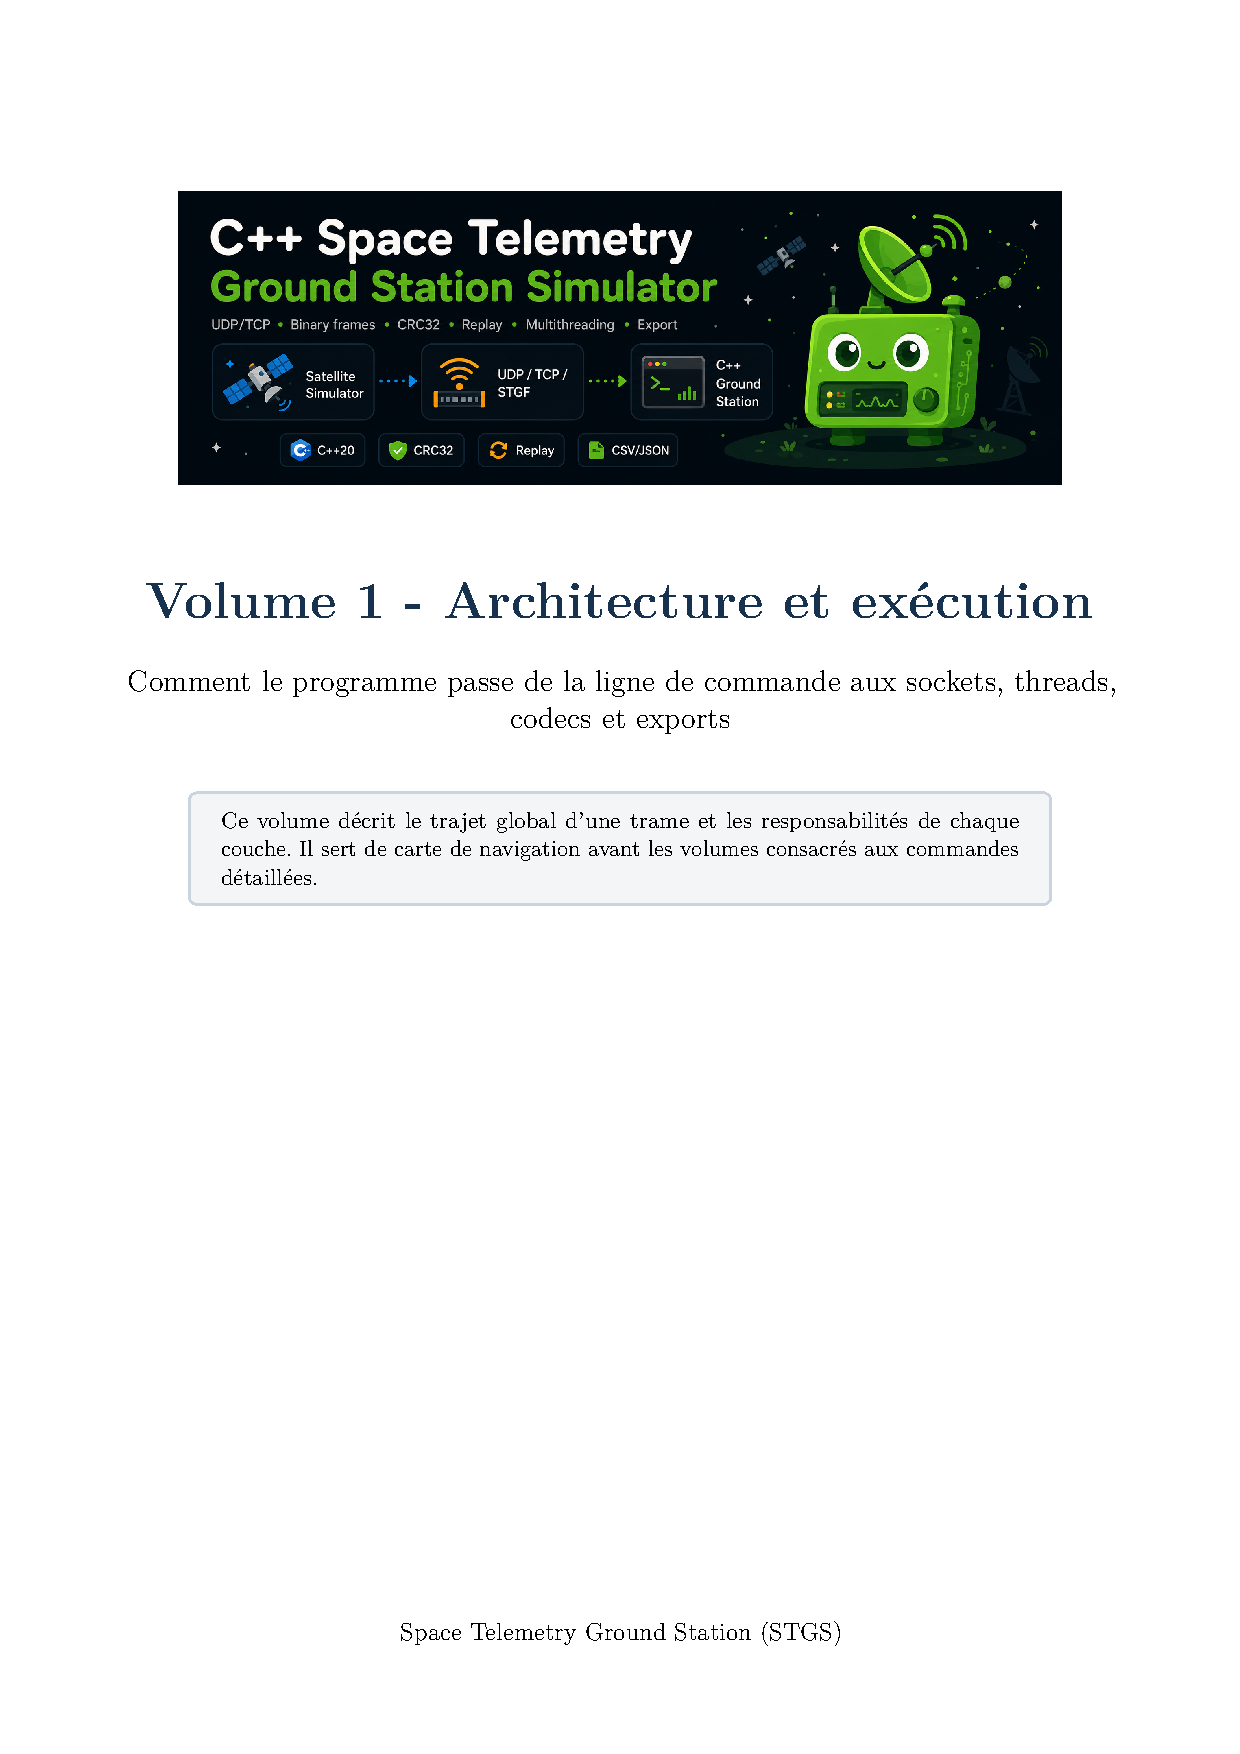
\includepdf[pages=-,pagecommand={}]{STGS_01_Architecture_et_execution.pdf}
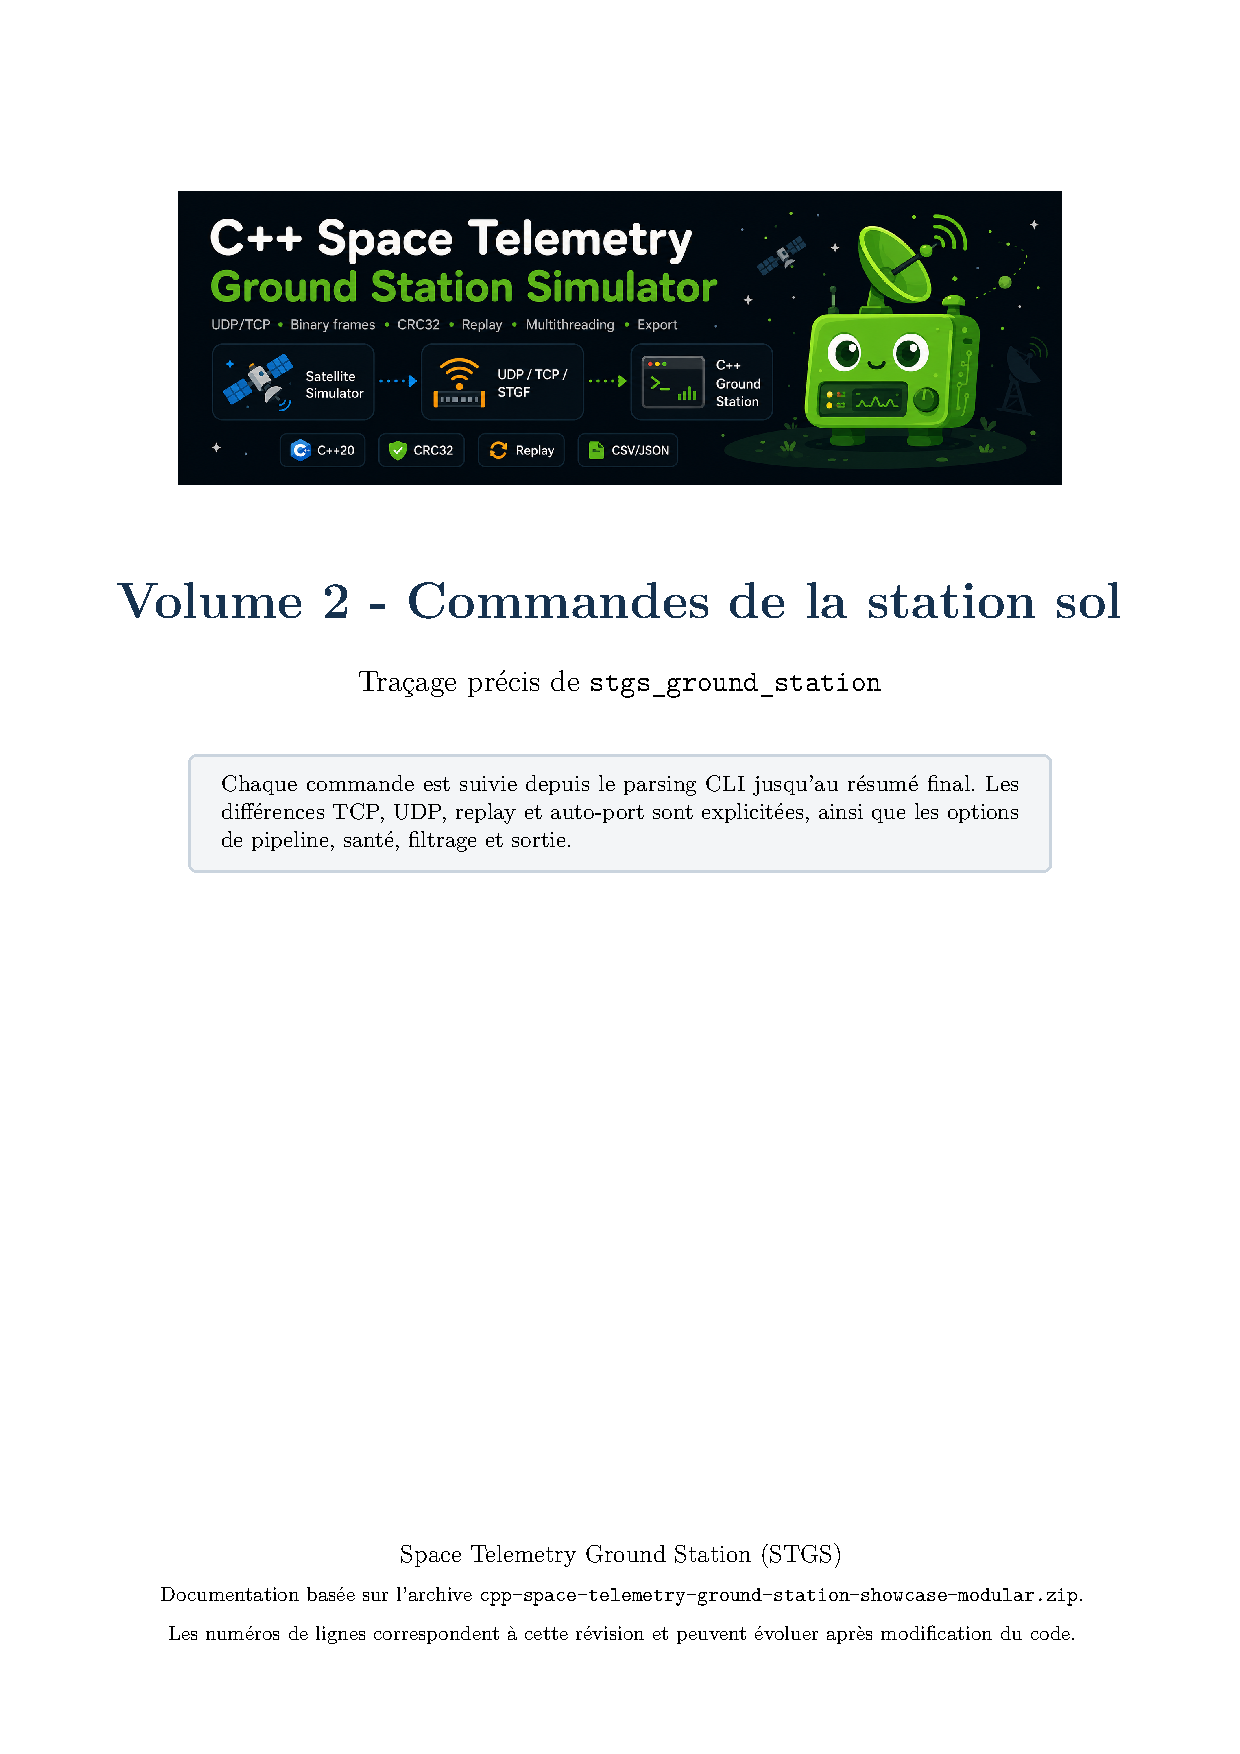
\includepdf[pages=-,pagecommand={}]{STGS_02_Commandes_station_sol.pdf}
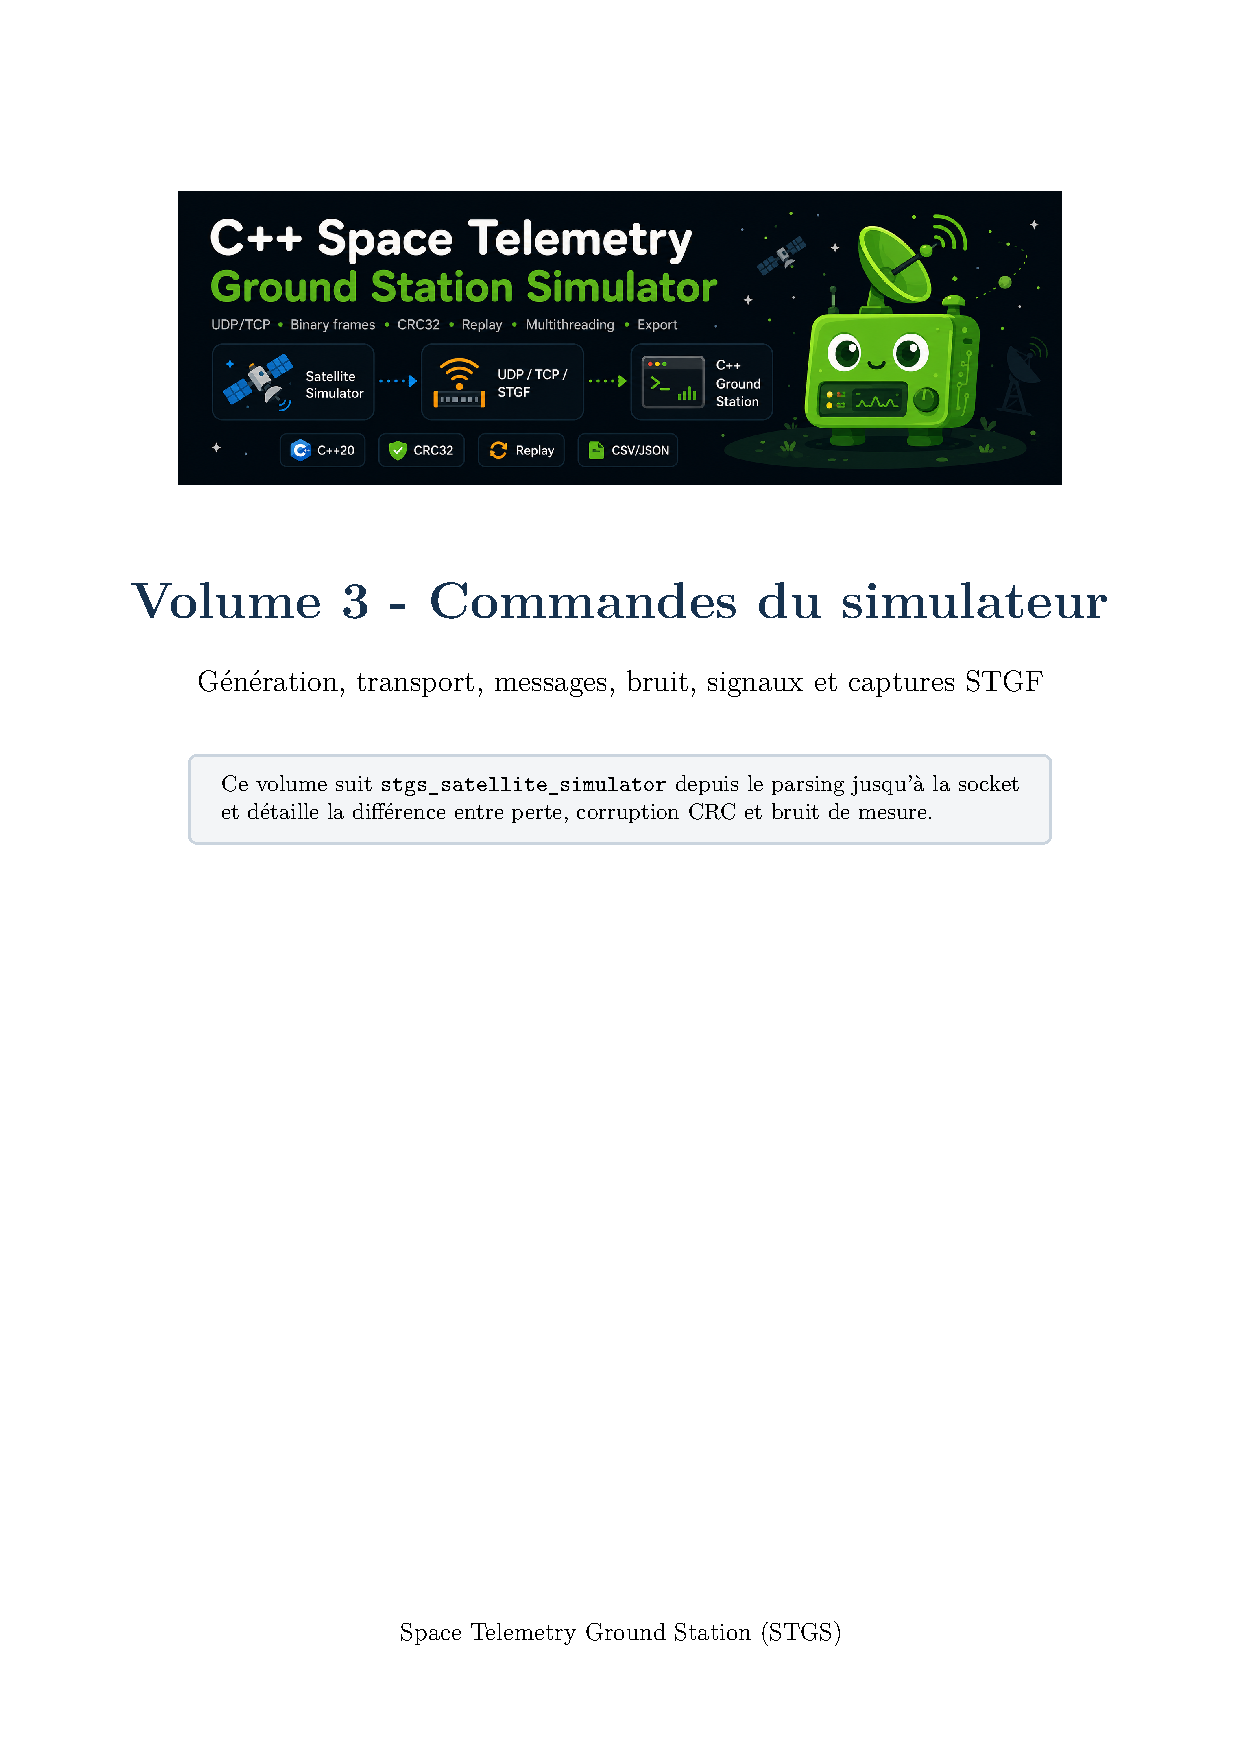
\includepdf[pages=-,pagecommand={}]{STGS_03_Commandes_simulateur.pdf}
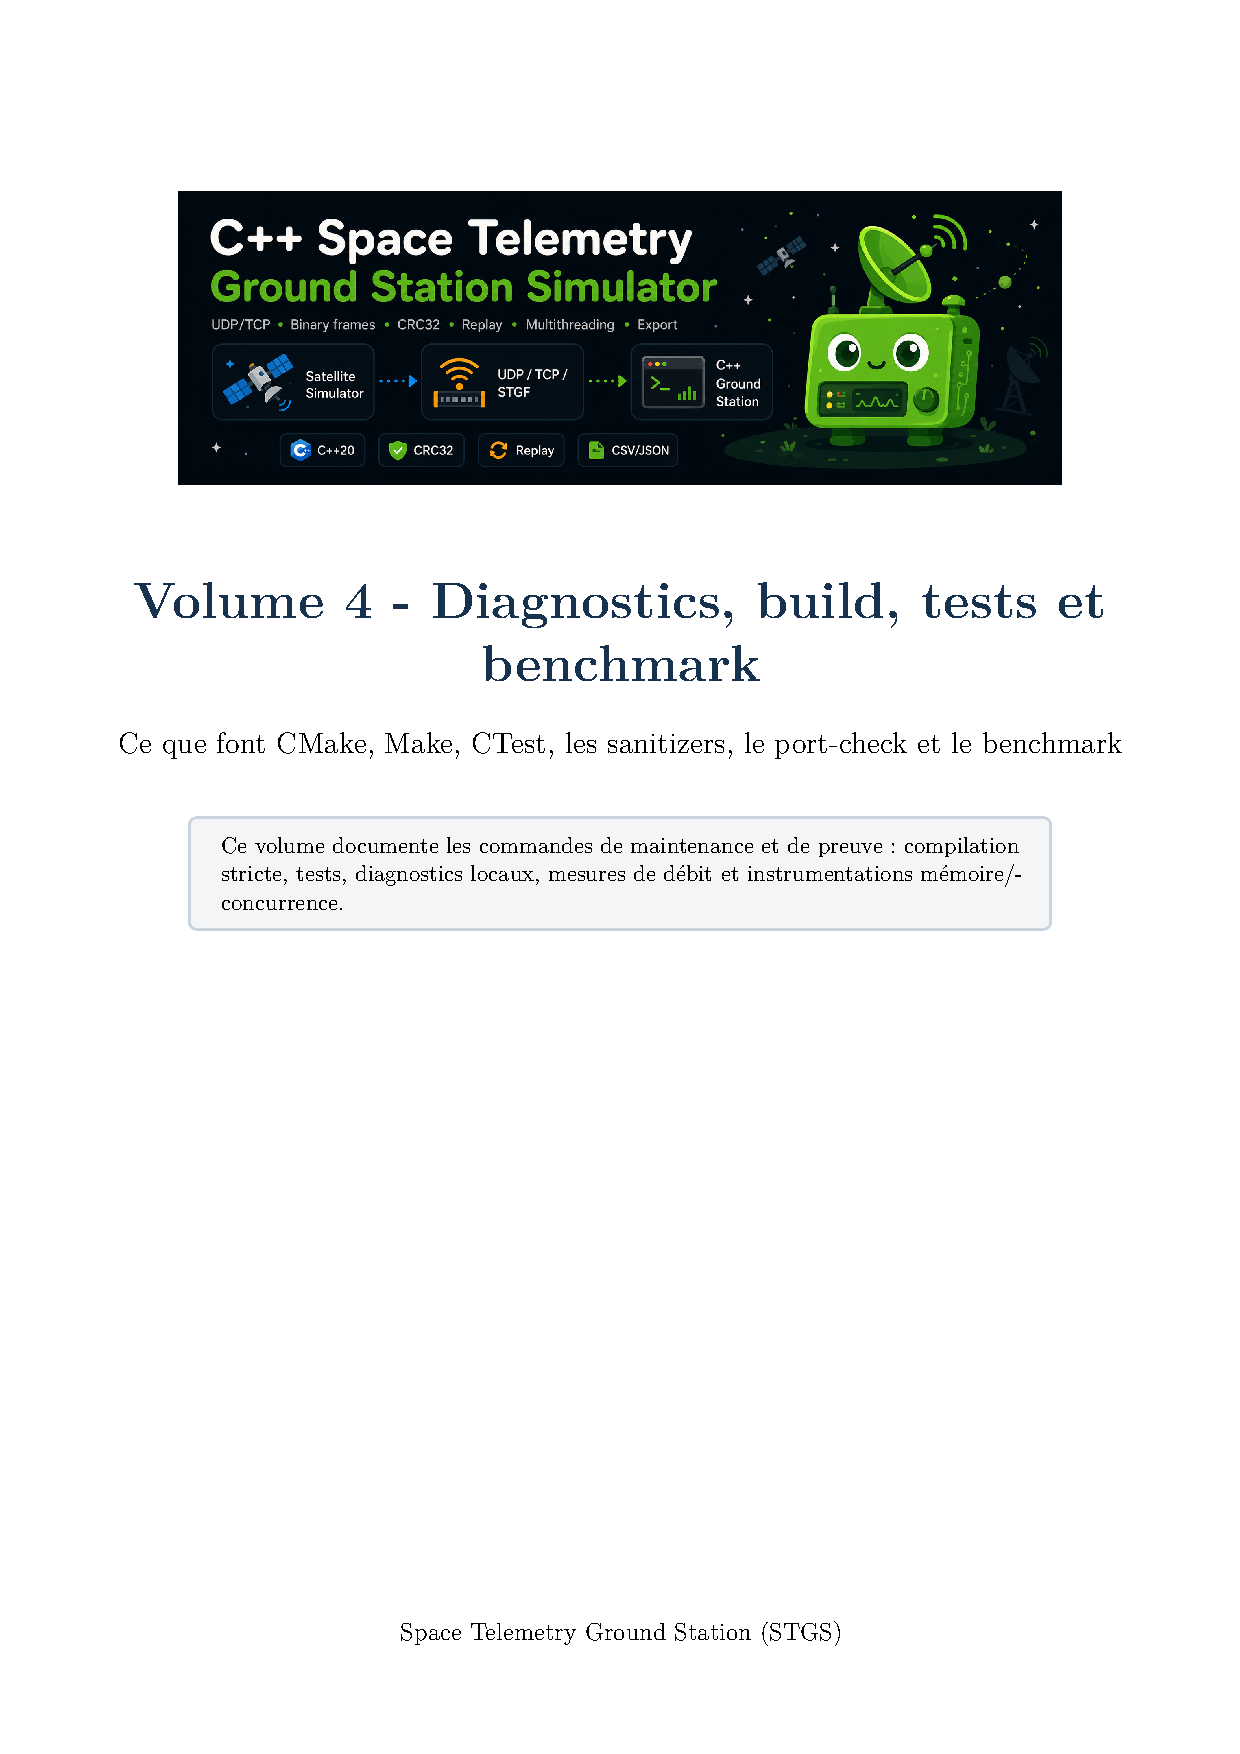
\includepdf[pages=-,pagecommand={}]{STGS_04_Diagnostics_build_tests_benchmark.pdf}
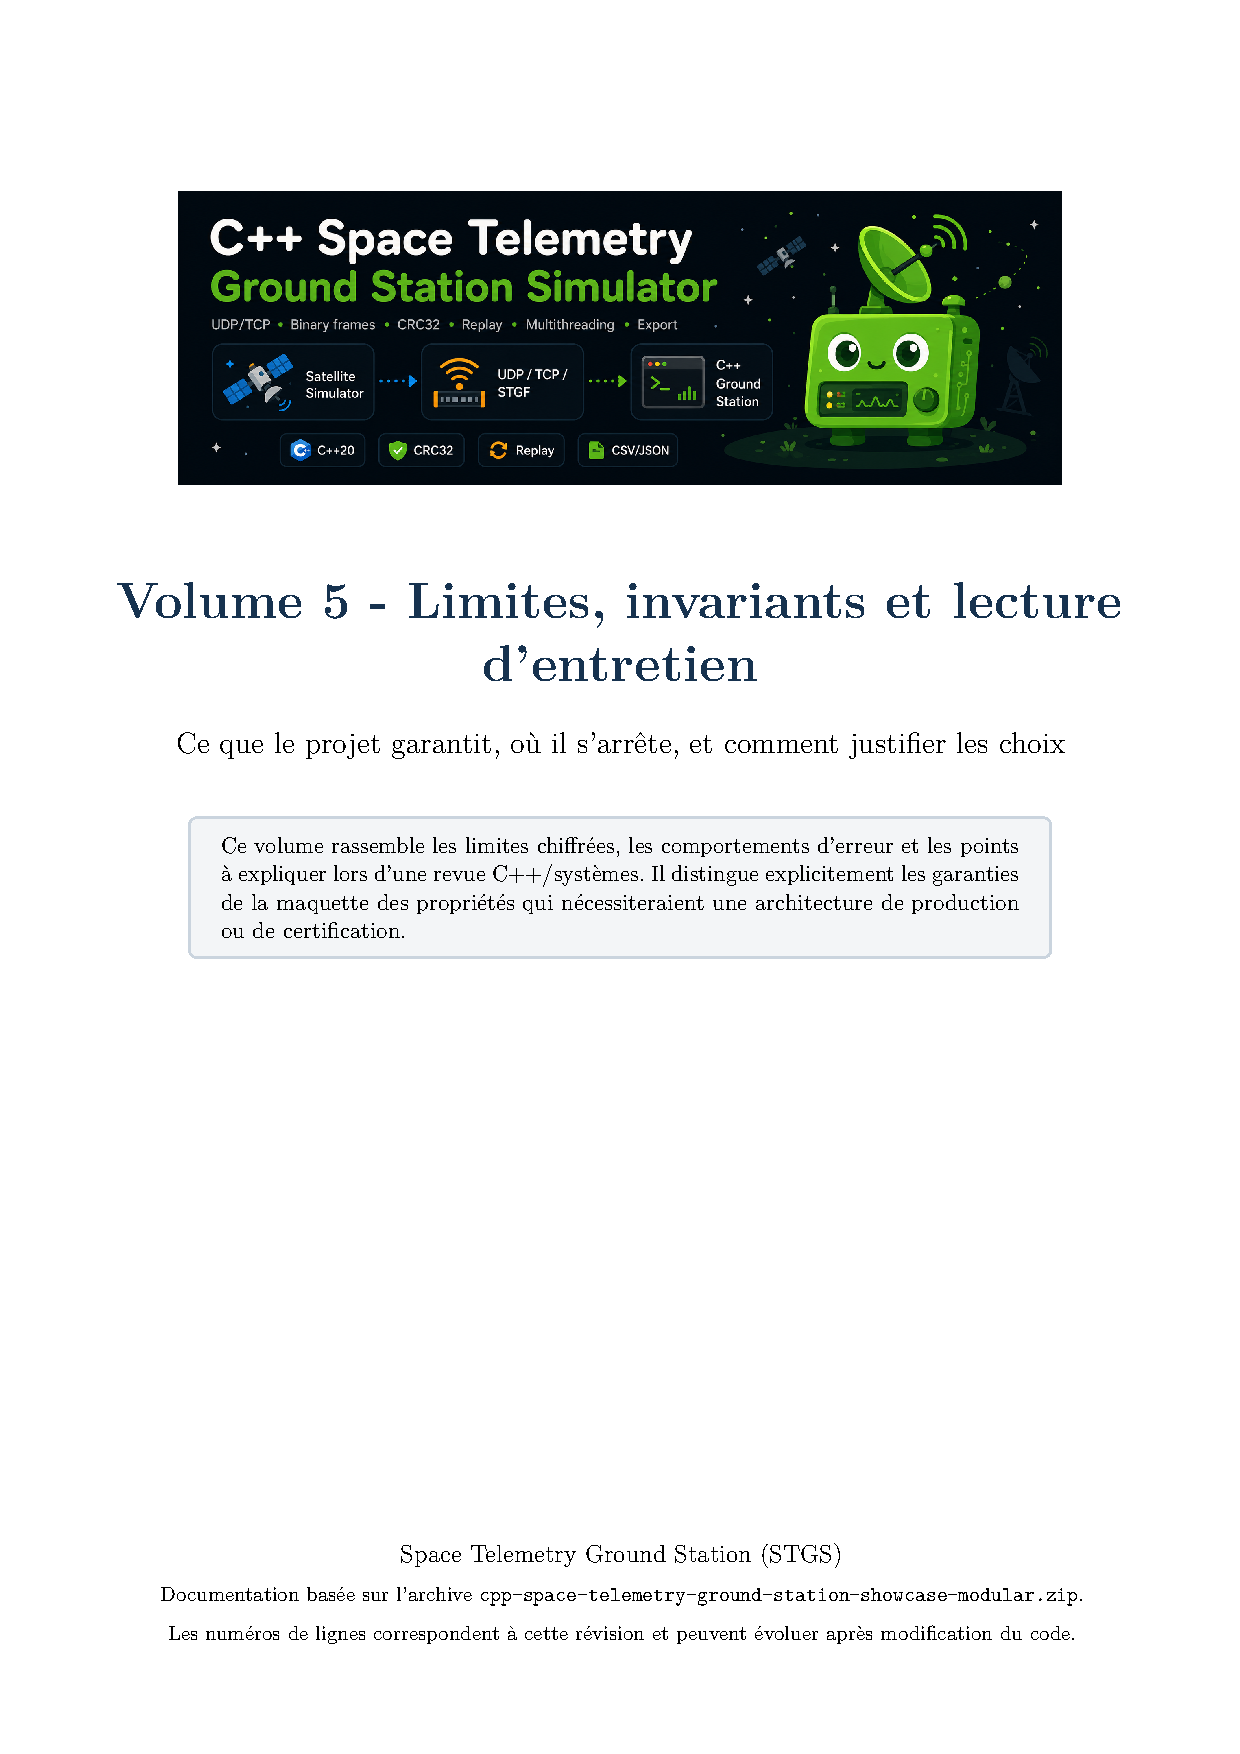
\includepdf[pages=-,pagecommand={}]{STGS_05_Limites_invariants_entretien.pdf}
\end{document}
